%!TEX root = ../thesis.tex

\chapter{Mobile App}
\label{sec:mobile_app}

Smart heating systems are on the uprise. More and more companies are trying to secure a spot in the market offering a variety of features in their control applications, which are mostly mobile or tablet based or even come with their own device. In this section we discuss the Android application we designed and implemented for users to control our heating system. We focused on keeping things simple because as we were researching some of the already existing systems we realized very quickly that the main issue is usability. The user is in almost all cases bombarded with features and extras and even though most of them would be very useful and effective, the average user will most likely be overwhelmed. The user interfaces we have seen are cluttered with buttons and options to finetune one's system. See Figure \ref{fig:smart_heating_apps} for some examples.

\begin{figure}[h]
	\begin{center}
		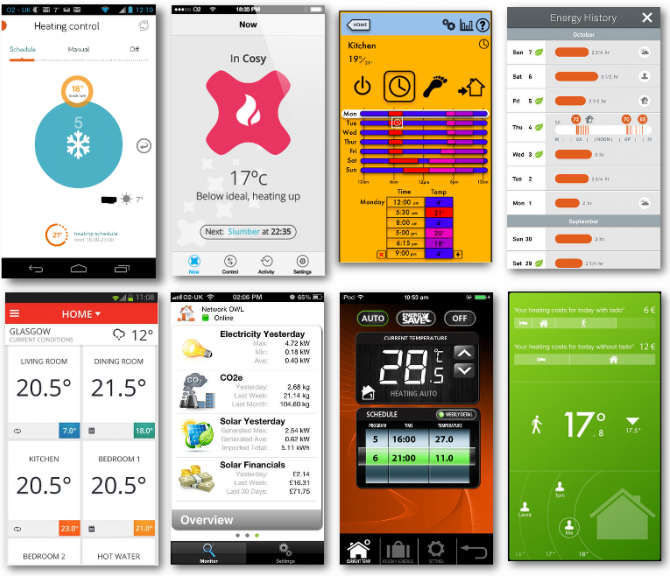
\includegraphics[width=0.8\textwidth]{images/smart_heating_apps.png}
	\end{center}
	\caption{Some examples of mobile applications for controlling smart heatings systems. Source: \url{https://cdn.recombu.com/media/digital/news/legacy/M13058/1397569835_w670_h576.png}}
	\label{fig:smart_heating_apps}
\end{figure}


\section{Use Cases}

We start by analyzing different use cases that an average user might run into and see what would happen in the application in these cases.

\begin{enumerate}
\item \textbf{User opens the application for the first time}

The user is presented with a welcome screen explaining how he can setup his heating system.
\item \textbf{etc..}

And so on..
\end{enumerate}

\subsection{Evaluation}

Uses cases 5 and 8 are neglected because of reasons.... Evaluate the use cases, explain what was solved and what wasn't and why it wasn't.

\section{Application flow}
See Figure \ref{fig:app_flow}.
\begin{figure}[h]
	\begin{center}
		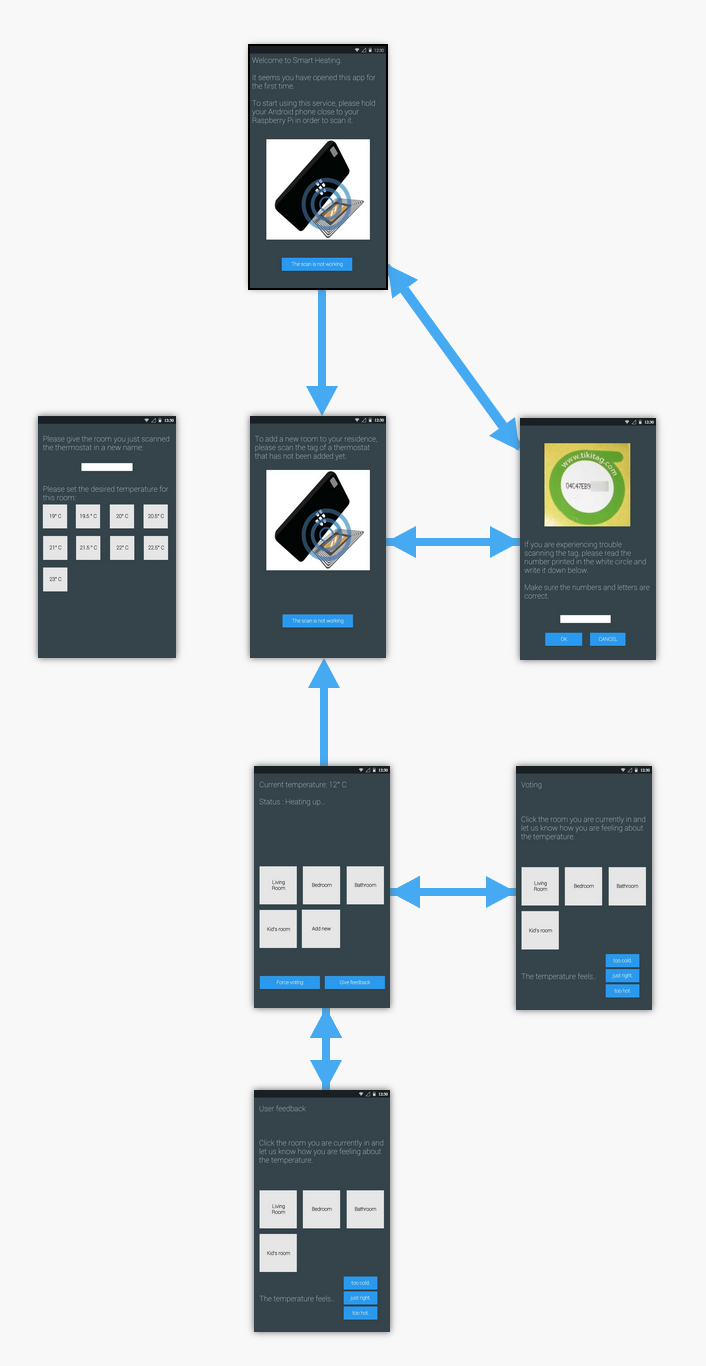
\includegraphics[width=0.8\textwidth]{images/app_flow.png}
	\end{center}
	\caption{The flow of the control application.}
	\label{fig:app_flow}
\end{figure}
\todo[inline]{Create and add app flow with actual screenshots of the app, also make it left-to-right}
